% Format teze zasnovan je na paketu memoir
% http://tug.ctan.org/macros/latex/contrib/memoir/memman.pdf ili
% http://texdoc.net/texmf-dist/doc/latex/memoir/memman.pdf
% 
% Prilikom zadavanja klase memoir, navedenim opcijama se podešava 
% veličina slova (12pt) i jednostrano štampanje (oneside).
% Ove parametre možete menjati samo ako pravite nezvanične verzije
% mastera za privatnu upotrebu (na primer, u b5 varijanti ima smisla 
% smanjiti 
\documentclass[12pt,oneside]{memoir} 
% Paket koji definiše sve specifičnosti master rada Matematičkog fakulteta
\usepackage[latinica,biblatex]{matfmaster} 
\usepackage{listings}
\usepackage{verbatim}
\usepackage{url}
\newtheorem{primer}{Primer}

\usepackage[latinica]{pangrami}

% Datoteka sa literaturom u BibTex tj. BibLaTeX/Biber formatu
\bib{literatura}

% Ime kandidata na srpskom jeziku (u odabranom pismu)
\autor{Ana Đorđević}
% Naslov teze na srpskom jeziku (u odabranom pismu)
\naslov{Automatsko generisanje test primera uz pomoć statičke analize i rešavača Z3}
% Godina u kojoj je teza predana komisiji
\godina{2017}
% Ime i afilijacija mentora (u odabranom pismu)
\mentor{dr Milena \textsc{Vujošević Janičić}, docent\\ Univerzitet u Beogradu, Matematički fakultet}
% Ime i afilijacija prvog člana komisije (u odabranom pismu)
\komisijaA{dr Filip \textsc{Marić}, vanredni profesor\\ Univerzitet u Beogradu, Matematički fakultet}
% Ime i afilijacija drugog člana komisije (u odabranom pismu)
\komisijaB{dr Milan \textsc{Banković}, docent \\ Univerzitet u Beogradu, Matematički fakultet}
% Ime i afilijacija trećeg člana komisije (opciono)
% \komisijaC{}
% Ime i afilijacija četvrtog člana komisije (opciono)
% \komisijaD{}
% Datum odbrane (odkomentarisati narednu liniju i upisati datum odbrane ako je poznat)
% \datumodbrane{}

% Apstrakt na srpskom jeziku (u odabranom pismu)
\apstr{%
}

% Ključne reči na srpskom jeziku (u odabranom pismu)
\kljucnereci{verifikacija softvera, testiranje softvera, SMT rešavači, Z3 rešavač, računarstvo}

\begin{document}
% ==============================================================================
% Uvodni deo teze
\frontmatter
% ==============================================================================
% Naslovna strana
\naslovna
% Strana sa podacima o mentoru i članovima komisije
\komisija
% Strana sa posvetom (u odabranom pismu)
\posveta{Mami i tati}
% Strana sa podacima o disertaciji na srpskom jeziku
\apstrakt
% Sadržaj teze
\tableofcontents*

% ==============================================================================
% Glavni deo teze
\mainmatter
% ==============================================================================

% ------------------------------------------------------------------------------
\chapter{Uvod}
% ------------------------------------------------------------------------------


% ------------------------------------------------------------------------------
\chapter{Rešavač Z3}
\label{chp:razrada}

Sistemi za analizu i verifikaciju softvera su veoma kompleksni. Njihovu osnovu predstavlja komponenta koja koristi logičke formule za opisivanja stanja i transformacija između stanja sistema. Opisivanje stanja sistema svodi se na proveravanje zadovoljivosti formula logike prvog reda. 
Proveravanje zadovoljivosti formula vrši se procedurama odlučivanja u odnosu na definisanu teoriju. Formalno, zadovoljivost u odnosu na teoriju (eng. Satisfiability Modulo Theory, skraćeno SMT) problem je odlučivanja zadovoljivosti u odnosu na osnovnu teoriju T opisanu u klasičnoj logici prvog reda sa jednakošću \cite{Barrett}. Alati koji se koriste za rešavanje ovog problema nazivaju se SMT rešavači. 
\par

Jedan od najpoznatijih SMT rešavača je rešavač Z3 kompanije Microsoft koji se koristi za proveru zadovoljivosti logičkih formula u velikom broju teorija \cite{EfficientSMTSolver}. Z3 se najčešče koristi kao podrška drugim alatima, pre svega alatima za analizu i verifikaciju softvera. Rešavač Z3 nudi interfejs za direktnu komunikaciju sa programskim jezicima C, C++ i Python. Pripada grupi SMT rešavača sa integrisanim procedurama odlučivanja.
\par
U ovoj glavi biće opisane osnove rešavača Z3 u delu \ref{sec:num1}. U delu \ref{sec:num2} biće opisane najvažnije teorije uključujući teoriju linearne aritmetike, teoriju nelinearne aritmetike, teoriju bitvektora i teoriju nizova. U delu \ref{sec:num3} opisani su podržani tipovi podataka.  


\section{Osnove rešavača}  \label{sec:num1}
Problem zadovoljivosti (eng. Satisfiability problem, skraćeno SAT) problem je odlučivanja da li za iskaznu formulu u konjunktivnoj normalnoj formi postoji valuacija u kojoj su sve njene 
klauze tačne \cite{Handbook}. 
Rešavači koji se koriste za rešavanje ovog problema nazivaju se SAT rešavači.   
Rešavač Z3 integriše SAT rešavač zasnovan na savremenoj DPLL proceduri i veliki broj teorija. 
Implementiran je u programskom jeziku C++. Šematski prikaz arhitekture \cite{EfficientSMTSolver} rešavača prikazan je na slici \ref{slika1}. 
\begin{figure}[!ht]\label{slika1}
  \centering
  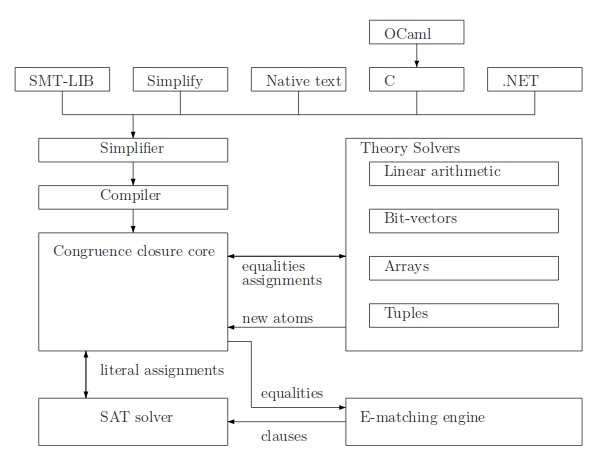
\includegraphics[width=1\textwidth]{arhitektura.png}
  \caption{Arhitektura rešavača Z3}
  \label{fig:arhitektura}
\end{figure}
\par
Formule prosleđene rešavaču se najpre procesiraju upotrebom simplifikacije. Simplifikacija primenjuje algebarska pravila redukcije kao što je \texttt{p $\land$ true $\vdash$ true}. Pored toga, ovim procesom se vrše odgovarajuće zamene kao što je \texttt{x=4 $\land$ q(x) $\vdash$ x=4 $\land$ q(4)}.
Nakon simplifikacije, kompajler formira apstraktno sintaksno stablo formula čiji su čvorovi simplifikovane formule (klauze). Zatim se jezgru kongruentnog zatvorenja (eng. Congruence closure core) prosleđuje apstraktno sintaksno stablo. Jezgro kongruentnog zatvorenja komunicira sa SAT rešavačem koji određuje istinitosnu vrednost klauza. 
\par
Ulazni format rešavača Z3 je definisan SMT-LIB 2.0 standardom. Standard definiše jezik logičkih formula čija se zadovoljivost proverava u odnosu na neku teoriju. Cilj standarda je obezbeđivanje zajedničkog jezika za sve SMT rešavače. 
\par
Interno, Z3 održava stek korisnički definisanih formula i deklaracija. Nazivamo ih tvrđenjima definisanih od strane korisnika. Komandom \texttt{push} kreira se novi opseg i čuva se trenutna veličina steka. Komandom \texttt{pop} uklanjaju se sva tvrđenja i deklaracije zadate posle push-a sa kojim se komanda uparuje. Komandom \texttt{assert} dodaje se formula na interni stek. Skup formula na steku je zadovoljiv ako postoji interpretacija u kojoj sve formule imaju istinitosnu vrednost tačno. Ova provera se vrši komandom \texttt{check-sat}. U slučaju zadovoljivosti vraća se \texttt{sat}, u slučaju nezadovoljivosti vraća se \texttt{unsat} a kada rešavač ne može da proceni da li je formula zadovoljiva ili ne vraća se \texttt{unknown}. Komandom \texttt{get-model} vraća se interpretacija u kojoj su sve formule na steku tačne. 
\par
Glavni gradivni blokovi formula su konstante, funkcije i relacije. Konstante su specijalan slučaj funkcija bez parametara. 

Relacije su funkcije koje vraćaju povratnu vrednost tipa Boolean. Funkcije mogu uzimati argumente tipa Boolean pa se na taj način relacije mogu koristiti kao argumenti funkcija. Za razliku od programskih jezika, funkcije logike prvog reda su totalne, tj. definisane su za sve vrednosti ulaznih parametara. Na primer, deljenje 0 je dozvoljeno, ali nije specifikovano šta ono predstavlja. Funkcije i konstantni simboli su neiterpretirani. Ovo je kontrast u odnosu na funkcije odgovarajućih teorija. Funkcija + ima standardnu interpretaciju u teoriji aritmetike. Neiterpretirane funkcije i konstante su maksimalno fleksibilne i dozvoljavaju bilo koju interpretaciju koja je u skladu sa ograničenjima. 

%\begin{primer} Kod demonstrira upotrebu neinterpretiranih tipova i funkcija %dokazivanjem identiteta: x = y => g(x) = g(y) upotrebom C++ API-ja. Formiramo %dva konstantna celobrojna izraza x i y i deklarišemo funkciju g sa jednim %argumentom. Dodajemo implikaciju, a zatim njenu negaciju prosleđujemo %rešavaču. Negacija implikacije je nezadovoljiva, pa je polazna formula validna %čime dokazujemo identitet.
%\begin{lstlisting}
%void dokazi_jednakost() {  
%    context c;
%    expr x      = c.int_const("x");
%    expr y      = c.int_const("y");
%    sort I      = c.int_sort();
%    func_decl g = function("g", I, I);  
%    solver s(c);
%    expr conjecture1 = implies(x == y, g(x) == g(y));
%    s.add(!conjecture1);
%    if (s.check() == unsat) 
%        std::cout << "dokazano";
%    else
%        std::cout << "ne moze se dokazati";
%}


%\end{lstlisting}
%\end{primer}

Komandom \texttt{declare-const} deklariše se konstanta odgovarajuće sorte (odgovara tipu promenljive u programskim jezicima). Sorta može biti parametrizovana i u tom slučaju su specifikovana imena njenih parametara. Specifikacija sorte vrši se naredbom \texttt{(define-sort [symbol] ([symbol]+)[sort])}.
Komandom \texttt{declare-fun} deklariše se funkcija. 


\begin{primer} Naredni kod demonstrira upotrebu konstanti i funkcija. U primeru se deklariše konstanta a celobrojnog tipa i funkcija f sa parametrima tipa Int i Bool i povratnom vrednošću tipa Int. Zatim se dodaju odgovarajuća ograničenja za konstantu a i funkciju f korišćenjem operatora poređenja. Rešavač Z3 pronalazi da je ovo tvrđenje zadovoljivo i daje prikazani model. 
\\ \\

\hspace{-0.7cm}
\begin{minipage}[b]{0.4\textwidth}
Formula prosleđena rešavaču:
(declare-const a Int)\\
(declare-fun f (Int Bool) Int)\\
(assert (> a 10))\\
(assert (< (f a true) 100))\\
(check-sat)\\
(get-model) \\
\end{minipage}
\hspace{2.4cm}
\begin{minipage}[t]{0.4\textwidth}
\vspace{-4.75cm}
Izlaz:
\\sat (model 
\\(define-fun a () Int 11) 
\\(define-fun f ((x!1 Int) (x!2 Bool)) Int 
\\(ite (and (= x!1 11) (= x!2 true)) 0 0)))
\end{minipage}
\end{primer}


Formula F je validna ako je vrednost valuacije true za bilo koje interpretacije funkcija i konstantnih simbola. Formula F je zadovoljiva ukoliko postoji evaluacija u kojoj je njena vrednost tačna. Da bismo odredili da li je formula F valjana, rešavač Z3 proverava da li je formula not F zadovoljiva. Ukoliko je negacija formule nezadovoljiva, onda je polazna formula validna. 

\begin{primer} Dokazivanje de Morganovog zakona dualnosti ispitivanjem validnosti formule: $\neg{(a \land b)} \Leftrightarrow (\neg{a} \lor \neg{b}) $ tako što se kao ograničenje dodaje negacija polazne formule. Z3 pronalazi da je negacija formule nezadovoljiva, pa je polazna formula tačna u svim interpretacijama. \\

\hspace{-0.7cm}
\begin{minipage}[b]{0.4\textwidth}
Formula prosleđena rešavaču:
\\(declare-const a Bool)
\\(declare-const b Bool)
\\(define-fun demorgan () Bool
\\    (= (and a b) (not (or (not a) (not b)))))
\\(assert (not demorgan))
\\(check-sat) 
\\(get-model)
\end{minipage}
\hspace{3.5cm}
\begin{minipage}[t]{0.4\textwidth}
\vspace{-5.35cm}
Izlaz:
\\unsat
\end{minipage}
\end{primer}
 
%Kao što je već napomenuto, rešavač Z3 nudi interfejs za direktnu komunikaciju %sa programskim jezicima. U daljem radu biće navedeni primeri korišćenjem C++ %API-ja.  
%\begin{primer} Dokazujemo De Morganov zakon dualnosti korišćenjem formule 
%$\neg{(a \land b)} \Leftrightarrow (\neg{a} \lor \neg{b}) $ korišćenjem C++ %API-ja. Rešavaču se prosleđuje negirana formula. Rešavač vraća %nezadovoljivost, čime pokazujemo da formula važi u svim interpretacijama.
%\begin{lstlisting}
%void demorgan() {
%    context c;
%    expr x = c.bool_const("a");
%    expr y = c.bool_const("b");
%    expr conjecture = !(a && b) == (!a || !b);
%    solver s(c);
%    // dodavanje negacije konjunkcije kao ogranicenja
%    s.add(!conjecture);
%    std::cout << s;
%    switch (s.check()) {
%    case unsat:   std::cout << "Formula je validna";
%    case sat:     std::cout << "Formula nije validna";
%    case unknown: std::cout << "Rezultat je nepoznat"; 
%    }
%}

%\end{lstlisting}
%\end{primer}

\section{Teorije} \label{sec:num2}
Teorije rešavača Z3 su opisane u okviru višesortne logike prvog reda sa jednakošću.  Definisanjem specifične teorije, uvode se restrikcije pri definisanju formula kao i podržanih relacija i operatora koje se na njih primenjuju. Na taj način, specijalizovane metode u odgovarajućoj teoriji mogu biti efikasnije implementirane u poređenju sa opštim slučajem. U nastavku će biti opisane teorija linearne aritmetike, teorija nelinearne aritmetike, teorija bitvektora i teorija nizova.

\subsection{Teorija linearne aritmetike} 

Rešavač Z3 sadrži procedure odlučivanja za linearnu aritmetiku nad celobrojnim i realnim brojevima. Dodatni materijali o procedurama odlučivanja linearne aritmetike dostupni su na \cite{FastLinearArithmetic}.
\par

U skladu sa standardom SMT-LIB 2.0, formule celobrojne linearne aritmetike konstruišu se korišćenjem funkcijskih simbola +, -, *, $\sim$ (unarna negacija), div i mod. Za funkcijske simbole div i mod, drugi operand mora biti različit od 0. 

U realnoj linearnoj aritmetici, interpretirani funkcijski simboli su +,- ,* i $\sim$(unarna negacija). Konstante se mogu porediti korišćenjem operatora =, <, <=, >, >=. 
\\
\par
Z3 rešavač ima podršku za celobrojne i realne konstante. Prethodno pomenutom komandom \texttt{declare-const} deklarišu se celobrojne i realne konstante. Rešavač ne vrši automatsku konverziju između celobrojnih i realnih konstanti. U tom slučaju koristi se funkcija \texttt{to-real} za konvertovanje celobrojnih u realne vrednosti.
Realne konstante treba da budu zapisane sa decimalnom tačkom.

\begin{primer} Naredni kod ilustruje pronalaženje interpretacija celobrojnih i realnih konstanti. Interpretacija se svodi na pridruživanje brojeva svakoj konstanti u slučaju zadovoljivosti formule. Ograničenja sadrže pomenute aritmetičke operatore. Rešavač zadovoljivost tvrđenja i dobijeni model prikazujemo u nastavku.\\ \\
\begin{minipage}[b]{0.4\textwidth}
Formula prosleđena rešavaču:
\\(declare-const a Int)
\\(declare-const b Int)
\\(declare-const c Int)
\\(declare-const d Real)
\\(declare-const e Real)
\\(assert (> e (+ (to\_real (+ a b)) 2.0)))
\\(assert (= d (+ (to\_real c) 0.5)))
\\(assert (> a b))
\\(check-sat)
\\(get-model)
\end{minipage}
\hspace{3.15cm}
\begin{minipage}[t]{0.4\textwidth}
\vspace{-7.2cm}
Izlaz:
\\sat 
\\(model
\\(define-fun b () Int 0) 
\\(define-fun a () Int 1) 
\\(define-fun e () Real 4.0) \\(define-fun c () Int 0) \\(define-fun d () Real (/ 1.0 2.0)))
\end{minipage}


\end{primer}


Takođe, postoji uslovni operator (if-then-else operator). Na primer,
izraz (ite (and (= x!1 11) (= x!2 false)) 21 0) ima vrednost 21 kada je promenljiva x!1 jednaka 11, a promenljiva x!2 ima vrednost False. U suprotnom, vraća se 0.

U slučaju deljenja, može se koristiti ite (if-then-else) operator i na taj način se može dodeliti interpretacija u slučaju deljenja nulom.
\par
Mogu se konstruisati novi operatori, korišćenjem define-fun konstruktora. Ovo je zapravo makro, pa će rešavač vršiti odgovarajuće zamene.
\begin{primer} Kod definiše operator deljenja tako da rezultat bude specifikovan i kada je delilac 0. Zatim se uvode dve konstante realnog tipa i primenjuje se definisani operator. Z3 rešavač pronalazi nezadovoljivost tvrđenja, s obzirom da operator mydiv vraća 0 pa relacija poređenja ne može biti tačna.\\ \\
\begin{minipage}[b]{0.4\textwidth}
Formula prosleđena rešavaču:
\\; definišemo da je x/0.0 == 0.0 za svako x
\\(define-fun mydiv ((x Real) (y Real)) Real
\\  (if (not (= y 0.0))
\\      (/ x y)
\\      0.0))
\\(declare-const a Real)
\\(declare-const b Real)
\\(assert (>= (mydiv a b) 1.0))
\\(assert (= b 0.0))
\\(check-sat)

\end{minipage}
\hspace{3cm}
\begin{minipage}[t]{0.4\textwidth}
\vspace{-7.85cm}
Izlaz:
\\unsat
\end{minipage}
\end{primer}

\subsection{Teorija nelinearne aritmetike} 

Formula predstavlja formulu nelinearne aritmetike ako je oblika (* t s), pri čemu t i s nisu linearnog oblika.
Nelinearna celobrojna aritmetika je neodlučiva, tj. ne postoji procedura koja za proizvoljan ulaz vraća odgovor sat ili unsat. U najvećem broju slučajeva, Z3 vraća kao rezultat unknown. Postoje nelinearni problemi za koje Z3 rešavač vraća odgovarajući model koristeći procedure odlučivanja zasnovana na Grebnerovim bazama.

\begin{primer} Rešavanje različitih nelinearnih problema sa celobrojnim i realnim konstantama. Z3 rešavač ne pronalazi uvek model za nelinearne probleme, ovde se za drugo tvrđenje vraća nezadovoljivost. Kada su prisutna samo nelinearna ograničenja nad realnim konstantama, Z3 koristi posebne metode odlučivanja. Ove metode korišćene su za dokazivanje trećeg tvrđenja.\\ \\
\begin{minipage}[b]{0.4\textwidth}
Formula prosleđena rešavaču:
\\(declare-const a Int)
\\(assert (> (* a a) 3))
\\(check-sat)
\\(get-model)
\\(declare-const b Real)
\\(declare-const c Real)
\\(assert (= (+ (* b b b) (* b c)) 3.0))
\\(check-sat)
\\(declare-const b Real)
\\(declare-const c Real)
\\(assert (= (+ (* b b b) (* b c)) 3.0))
\\(check-sat)
\\(get-model)

\end{minipage}
\hspace{2.6cm}
\begin{minipage}[t]{0.4\textwidth}
\vspace{-9.75cm}
Izlaz:
\\sat 
\\(model 
\\(define-fun a () Int (-8)) ) 
\\unsat 
\\sat (
\\model 
\\(define-fun b () Real (/ 1.0 8.0)) 
\\(define-fun c () Real (/ 1535.0 64.0)))
\end{minipage}
\end{primer}

\subsection{Teorija bitvektora} 
Za razliku od programskih jezika, kao što su C, C++ i Java gde ne postoji razlika između označenih i neoznačenih bitvektora, rešavač Z3 ih tretira na različite načine. Teorija bitvektora ima na raspolaganju različite verzije aritmetičkih operacija za označene i neoznačene brojeve. Više materijala o procedurama odlučivanja za teoriju bitvektora može se naći na \cite{DPBitvector}.
\par
Z3 podržava vektore proizvoljne dužine. (\_ BitVec n) je sorta bitvektora čija je dužina n. Bitvektor literali se mogu definisati koristeći binarnu, decimalnu ili heksadecimalnu notaciju. U binarnom i heksadecimalnom slučaju, veličina bitvektora je određena brojem karaktera. Na primer, literal \#b010 u binarnom formatu je bitvektor dužine 3, a literal \#x0a0 u heksadecimalnom formatu je bitvektor veličine 12. Veličina bitvektora mora biti specifikovana u decimalnom formatu. Na primer, reprezentacija (\_ bv10 32) je bitvektor dužine 32 sa vrednošću 10. Podrazumevano, Z3 predstavlja bitvektore u heksadecimalnom formatu ukoliko je dužina bitvektora umnožak broja 4 a u suprotnom u binarnom formatu. Komanda 
(set-option :pp.bv-literals false) se može koristiti za predstavljanje literala bitvektora u decimalnom formatu. 
\begin{primer} Navodimo različite načine predstavljanja bitvektora. Ukoliko zapis počinje sa \#b, bitvektor se zapisuje u binarnom formatu. Ukoliko zapis počinje sa \#x, bitvektor se zapisuje u heksadecimalnom formatu. U oba slučaja, nakon specifikacije formata, zapisuje se dužina vektora. Drugi način zapisa počinje skraćenicom bv, navođenjem vrednosti i na kraju dužine. \\\\
\begin{minipage}[b]{0.4\textwidth}
Formula prosleđena rešavaču:
\\(display \#b0100)
\\(display (\_ bv20 8))
\\(display (\_ bv20 7))
\\(display \#x0a) 
\\(set-option :pp.bv-literals false)
\\(display \#b0100)
\\(display (\_ bv20 8))
\\(display (\_ bv20 7))
\\(display \#x0a)
\end{minipage}
\hspace{2.5cm}
\begin{minipage}[t]{0.4\textwidth}
\vspace{-5.9cm}
Izlaz:
\\\#x4 
\\\#x14 
\\\#b0010100 
\\\#x0a 
\\(\_ bv4 4) 
\\(\_ bv20 8) 
\\(\_ bv20 7) 
\\(\_ bv10 8)
\end{minipage}


\end{primer}


Za rad sa bitvektorima, definisane su operacije sabiranja, oduzimanja, negacije, množenja, izračunavanja modula pri deljenju, šiftovanje u levo kao i označeno i neoznačeno šifrovanje u desno. Podržane su sledeće logičke operacije nad bitovima: disjunkcija, konjunkcija, unarna negacija, negacija konjunkcije i negacija disjunkcije. Definisane su različite relacije nad bitvektorima kao što su <=, <, >=, > pri čemu su podržane i označene i neoznačene varijante pa se poređenje izvršava na različite načine. 


\begin{primer} Ilustracija podržanih aritmetičkih operacija nad bitvektorima uklučujući sabiranje, oduzimanje, unarnu negaciju, množenje, računanje modula, šiftovanje ulevo, neoznačeno (logičko) šiftovanje udesno i označeno (aritmetičko) šiftovanje udesno.
\\\\
\begin{minipage}[b]{0.5\textwidth}
Formula prosleđena rešavaču:
\\(simplify (bvadd \#x07 \#x03)) 
\\(simplify (bvsub \#x07 \#x03))
\\(simplify (bvneg \#x07)) 
\\(simplify (bvmul \#x07 \#x03)) 
\\(simplify (bvsmod \#x07 \#x03)) 
\\(simplify (bvshl \#x07 \#x03)) 
\\(simplify (bvlshr \#xf0 \#x03)) 
\\(simplify (bvashr \#xf0 \#x03)) 
\\(simplify (bvor \#x6 \#x3)) 
\\(simplify (bvand \#x6 \#x3))  
\\(simplify (bvnot \#x6)) 
\\(simplify (bvnand \#x6 \#x3)) 
\\(simplify (bvnor \#x6 \#x3)) 
\\(simplify (bvxnor \#x6 \#x3)) 

\end{minipage}
\hspace{2.5cm}
\begin{minipage}[b]{0.5\textwidth}
Izlaz:
\\\#x0a 
\\\#x04 
\\\#xf9 
\\\#x15 
\\\#x01 
\\\#x38 
\\\#x1e 
\\\#xfe
\\\#x7 
\\\#x2 
\\\#x9 
\\\#xd 
\\\#x8 
\\\#xa
\end{minipage}

\end{primer}


\begin{primer} Naredni kod dokazuje validnost De Morganovog zakona korišćenjem bitvektora. Deklarišu se dve konstante predstavljene bitvektorima dužine 64 a zatim se dodaje negacija formule i ispituje se njena zadovoljivost. Rešavač Z3 vraća unsat, negacija formule je nezadovoljiva.
Odavde zaključujemo da je polazna formula valjana.
\\ \\
\hspace{9.5cm}
\begin{minipage}[t]{0.5\textwidth}
Formula prosleđena rešavaču:
\\(declare-const x (\_ BitVec 64))
\\(declare-const y (\_ BitVec 64))
\\(assert 
\\(not (= (bvand (bvnot x) (bvnot y)) (bvnot (bvor x y)))))
\\(check-sat)
\\(get-model)
\end{minipage}
\hspace{2.5cm}
\begin{minipage}[t]{0.5\textwidth}
Izlaz:
\\unsat
\end{minipage}
\end{primer}


Postoji brz način da se proveri da li su brojevi fiksne dužine stepeni dvojke. 
Ispostavlja se da je bitvektor x stepen dvojke ako i samo ako je vrednost izraza
x \& (x - 1) jednaka 0.
\begin{primer} Provera da li je broj stepen dvojke vrši se definisanjem funkcije korišćenjem prethodno pomenute jednakosti. Dodaje se negacija ove jednakosti kao tvrđenja i vrši se proveravanje za bitvektore vrednosti 0, 1, 2, 4 i 8. U svim slučajevima brojevi su stepeni dvojke pa Z3 rešavač vraća nezadovoljivost.\\ \\
\begin{minipage}[b]{0.5\textwidth}
Formula prosleđena rešavaču:
\\(define-fun is-power-of-two 
\\((x (\_ BitVec 4))) Bool 
\\(= \#x0 (bvand x (bvsub x \#x1))))
\\(declare-const a (\_ BitVec 4))
\\(assert 
\\ (not (= (is-power-of-two a) 
\\         (or (= a \#x0) 
\\             (= a \#x1) 
\\             (= a \#x2) 
\\             (= a \#x4) 
\\             (= a \#x8)))))
\\(check-sat)
\\(get-model)
\end{minipage}
\hspace{2.5cm}
\begin{minipage}[t]{0.5\textwidth}
\vspace{-8.35cm}
Izlaz:
\\unsat
\end{minipage}
\end{primer}

\begin{primer} Ilustracija podržanih relacija nad bitvektorima. Podržane relacije uključuju neoznačene i označene verzije za operatore <, <=, > i >=. U nastavku slede pomenuti operatori primenom na dva operanda i njihove vrednosti kao izlaze.
\\ \\ 
\begin{minipage}[b]{0.5\textwidth}
Formula prosleđena rešavaču:
\\(simplify (bvule \#x0a \#xf0))  
\\(simplify (bvult \#x0a \#xf0))  
\\(simplify (bvuge \#x0a \#xf0))  
\\(simplify (bvugt \#x0a \#xf0))  
\\(simplify (bvsle \#x0a \#xf0)) 
\\(simplify (bvslt \#x0a \#xf0))  
\\(simplify (bvsge \#x0a \#xf0))  
\\(simplify (bvsgt \#x0a \#xf0))

\end{minipage}
\hspace{2cm} 
\begin{minipage}[t]{0.5\textwidth}
\vspace{-5.25cm}
Izlaz:
\\true 
\\true 
\\false 
\\false 
\\false 
\\false 
\\true 
\\true
\end{minipage}


\end{primer}


\begin{primer} Ilustracija označenog i neoznačenog poređenja bitvektora. Označeno poređenje, kao što je bvsle, uzima u obzir znak bitvektora za poređenje, dok neoznačeno poređenje tretira bitvektor kao prirodan broj. Z3 rešavač pronalazi da je tvrđenje zadovoljivo i daje prikazani model.
\\ \\
\begin{minipage}[b]{0.5\textwidth}
Formula prosleđena rešavaču:
\\(declare-const a (\_ BitVec 4))
\\(declare-const b (\_ BitVec 4))
\\(assert (not (= (bvule a b) (bvsle a b)))
\\(check-sat)
\\(get-model)
\end{minipage}
\hspace{1.15cm} 
\begin{minipage}[t]{0.5\textwidth}
\vspace{-3.4cm}
Izlaz:
\\sat 
\\(model 
\\(define-fun b () (\_ BitVec 4) \#xe) 
\\(define-fun a () (\_ BitVec 4) \#x0)
\\)
\end{minipage}


\end{primer}
Svojstvo da Z3 različito tretira označene i neoznačene bitvektore ilustrovano je  primerom.
 
%\begin{lstlisting}
%/*
% Primer sa bitvektorom pokazuje razliku u koriscenju oznacenog i neoznacenog %poredjenja
%*/
%void bitvector_example1() {

%    context c;
%    expr x = c.bv_const("x", 32);
    
%    // koriscenje oznacenog <=
%    prove((x - 10 <= 0) == (x <= 10));

%    // koriscenje neoznacenog <=
%    prove(ule(x - 10, 0) == ule(x, 10));
%}

%\end{lstlisting}

\subsection{Teorija nizova} 
Osnovnu teoriju nizova karakterisu select i store naredbe. 
Komandom (select a i) vraća se vrednost na poziciji i u nizu a, a izraz (store a i v) formira novi niz, identičan nizu a pri čemu se na poziciji i nalazi vrednost v.
Z3 sadrži procedure odlučivanja za osnovnu teoriju nizova.
Dva niza su jednaka ukoliko su vrednosti elemenata sa odgovarajućim indeksima jednake.
 
\begin{primer} Definišemo tri konstante x, y i z celobrojnog tipa. Neka je a1 niz celobrojnih vrednosti. Tada je ograničenje (and (= (select a1 x) x) (= (store a1 x y) a1)) zadovoljivo kada je element niza a na poziciji x jednak definisanoj konstanti x i u slučaju kada su konstante x i y jednake.
Rešavač Z3 vraća zadovoljivost zadatog tvrđenja i odgovarajući model.
 \\ \\
\begin{minipage}[b]{0.5\textwidth}
Formula prosleđena rešavaču:
\\(declare-const x Int)
\\(declare-const y Int)
\\(declare-const z Int)
\\(declare-const a1 (Array Int Int))
\\(assert (= (select a1 x) x))
\\(assert (= (store a1 x y) a1))
\\(check-sat)
\\(get-model)
\end{minipage}
\hspace{1.3cm} 
\begin{minipage}[t]{0.5\textwidth}
\vspace{-5.4cm}
Izlaz:
\\sat
\\(model 
\\(define-fun y () Int 1)
\\(define-fun a1 () (Array Int Int)
\\(\_ as-array k!0))
\\(define-fun x () Int 1)
\\(define-fun k!0 ((x!1 Int)) Int
\\    (ite (= x!1 1) 1
\\      0))
)

\end{minipage}
\end{primer} 
 

\subsection{Konstantni nizovi}

Nizovi koji sadrže konstantne vrednosti mogu se specifikovati koristeći const konstrukciju. Upotrebom const konstrukcije Z3 ne može da odluči kog tipa su elementi niza pa se on mora eksplicitno navesti. Interpretacija nizova je slična interpretaciji funkcija. Z3 koristi konstrukciju (\_ as-array f) za određivanje interpretacije niza. Ako je niz a jednak rezultatu konstrukcije (\_ as-array f), tada za svaki indeks i, vrednost (select a i) odgovara vrednosti (f i). 

\begin{primer} Defnišemo konstantni niz all1 celobrojnog tipa i dve celobrojne konstante a i i. Uvodimo ograničenje da niz all1 sadrži samo jedinice. Z3 pronalazi da je ovo tvrdjenje zadovoljivo, i daje prikazani model.\\ \\
\begin{minipage}[b]{0.5\textwidth}
Formula prosleđena rešavaču:
\\(declare-const all1 (Array Int Int))
\\(declare-const a Int)
\\(declare-const i Int)
\\(assert (= all1 ((as const (Array Int Int)) 1)))
\\(assert (= a (select all1 i)))
\\(check-sat)
\\(get-model)
\end{minipage}
\hspace{1.5cm} 
\begin{minipage}[b]{0.5\textwidth}
Izlaz:
\\sat 
\\(model 
\\(define-fun all1 () (Array Int Int) 
\\(\_ as-array k!0)) 
\\(define-fun i () Int 0) 
\\(define-fun a () Int 1) 
\\(define-fun k!0 ((x!0 Int)) Int 
\\(ite (= x!0 0) 1 1)) )
\end{minipage}
\end{primer}

Primena map funkcije na nizove
Z3 nudi parametrizovanu funkciju map na nizove. Omogućava primenu proizvoljnih funkcija na sve elemente niza.
\begin{primer} Definišemo dva konstantna niza a i b tipa Boolean i dokazujemo da važi svojstvo $\neg{(a \land b)} \Leftrightarrow (\neg{a} \lor \neg{b}) $ primenom na sve elemente nizova a i b korišćenjem funkcije map. Kao ograničenje dodajemo negaciju prethodno navedene formule. Rešavaš Z3 vraća nezadovoljivost negirane formule, odakle zaključujemo da je polazna formula validna.\\ \\
\begin{minipage}[b]{0.5\textwidth}
Formula prosleđena rešavaču:
\\(define-sort Set (T) (Array T Bool))
\\(declare-const a (Set Int))
\\(declare-const b (Set Int))
\\(assert (not (= ((\_ map and) a b) 
\\((\_ map not) 
\\((\_ map or) ((\_ map not) b) ((\_ map not) a))))))
\\(check-sat)
\end{minipage}
\hspace{2.5cm} 
\begin{minipage}[t]{0.5\textwidth}
\vspace{-5.3cm}
Izlaz:
\\unsat 
\end{minipage}
\end{primer}

\section{Tipovi podataka} \label{sec:num3}

Algebarski tipovi podataka omogućavaju specifikaciju uobičajnih struktura podataka. Slogovi i torke su specijalne vrste algebarskih tipova podataka kao i skalari (enumeracijski tipovi). Primena algebarskih tipova podataka može se generalizovati. Mogu se koristiti za specifikovanje konačnih lisi, stabala i rekurzivnih struktura. 
\subsection{Slogovi}
Slog se specifikuje kao tip podataka sa jednim konstruktorom i proizvoljnim brojem elemenata sloga. Sistem ne dozvoljava proširivanje slogova. Važi svojstvo da su dva sloga jednaka samo ako su im svi argumenti jednaki.

\begin{primer} Pokazujemo svojstvo da su dva sloga jednaka ako i samo ako su im svi argumenti jednaki. Uvodimo parametarski tip Pair, sa konstruktorom mk-pair i dva argumenta kojima se može pristupiti koristeći selektorske funkcije first i second. Definišemo dva sloga p1 i p2, čija su oba podatka celobrojnog tipa. Dodajemo ograničenja da su slogovi p1 i p2 jednaki kao i ograničenje koje se odnosi na drugi element sloga. Rešavač Z3 u prvom slučaju vraća zadovoljivost formule i odgovarajući model. Dodavanjem ograničenja da prvi elementi slogova nisu jednaki korišćenjem selektorske funkcije first, tvrđenje postaje nezadovoljivo.
\\ \\
\begin{minipage}[b]{0.5\textwidth}
Formula prosleđena rešavaču:
\\(declare-datatypes (T1 T2) 
\\((Pair (mk-pair (first T1) (second T2)))))
\\(declare-const p1 (Pair Int Int))
\\(declare-const p2 (Pair Int Int))
\\(assert (= p1 p2))
\\(assert (> (second p1) 20))
\\(check-sat)
\\(get-model)
\\(assert (not (= (first p1) (first p2))))
\\(check-sat)
\end{minipage}
\hspace{2cm} 
\begin{minipage}[t]{0.5\textwidth}
\vspace{-6.5cm}
Izlaz:
\\sat 
\\(model 
\\(define-fun p1 () (Pair Int Int) 
\\(mk-pair 0 21)) 
\\(define-fun p2 () (Pair Int Int) 
\\(mk-pair 0 21)) )
\\unsat
\end{minipage}

\end{primer}
\subsection{Skalari (tipovi enumeracije)}

Sorta skalara je sorta konačnog domena. Elementi konačnog domena se tretiraju kao različite konstante. Na primer, sorta S je skalarni tip sa tri vrednosti A, B i C. Moguće je da tri konstante sorte S budu različite. Ovo svojstvo ne može važiti u slučaju četiri konstante.

\begin{primer} Prilikom deklaracije skalarnog tipa podataka, navodi se broj različitih elemenata domena, u ovom primeru tri i pokazuje se nezadovoljivost tvrđenja sa četiri različita elementa domena. \\ \\
\begin{minipage}[b]{0.5\textwidth}
Formula prosleđena rešavaču:
\\(declare-datatypes () ((S A B C)))
\\(declare-const x S)
\\(declare-const y S)
\\(declare-const z S)
\\(declare-const u S)
\\(assert (distinct x y z))
\\(check-sat)
\\(assert (distinct x y z u))
\\(check-sat)
\end{minipage}
\hspace{3cm} 
\begin{minipage}[t]{0.5\textwidth}
\vspace{-5.9cm}
Izlaz:
\\sat 
\\(model 
\\(define-fun z () S A) 
\\(define-fun y () S B) 
\\(define-fun x () S C) ) 
\\unsat
\end{minipage}
\end{primer}

\subsection{Rekurzivni tipovi podataka}

Deklaracija rekurzivnog tipa podataka uključuje sebe direktno kao komponentu. Standardni primer rekurzivnog tipa podataka je lista. Parametrizovana lista može se definisati na sledeći način:\\
(declare-datatypes (T) ((Lst nil (cons (hd T) (tl Lst)))))
\\(declare-const l1 (Lst Int))
\\(declare-const l2 (Lst Bool))
\par
Postoji podrška za rekurzivni tip podataka korišćenjem ključne reči List. 
Prazna lista se definiše korišćenjem reči nil a konstruktor insert se koristi za formiranje novih lista. Selektori head i tail se definišu na uobičajan način.

\begin{primer} Deklarišemo tri liste l1,l2 i l3 sa celobrojnim vrednostima, kao i celobrojnu konstantu x. Dodaju se ograničenja za prve i poslednje elemente liste korišćenjem selektora. 
\\ \\
\begin{minipage}[b]{0.5\textwidth}
Formula prosleđena rešavaču:
\\(declare-const l1 (List Int))
\\(declare-const l2 (List Int))
\\(declare-const x Int)
\\(assert (not (= l1 nil)))
\\(assert (not (= l2 nil)))
\\(assert (= (head l1) (head l2)))
\\(assert (not (= l1 l2)))
\\(assert (= l3 (insert x l2)))
\\(assert (> x 100))
\\(check-sat)
\\(get-model)
\\(assert (= (tail l1) (tail l2)))
\\(check-sat)
\end{minipage}
\hspace{2.2cm}
\begin{minipage}[t]{0.5\textwidth}
\vspace{-8.45cm}
Izlaz:
\\sat 
\\(model 
\\(define-fun l3 () (List Int) 
\\(insert 101 
\\(insert 0 (insert 1 nil)))) 
\\(define-fun x () Int 101) 
\\(define-fun l1 () (List Int) 
\\(insert 0 nil)) 
\\(define-fun l2 () (List Int) 
\\(insert 0 (insert 1 nil)))) 
\\unsat
\end{minipage}


\end{primer}

U prethodnom primeru, uvodi se ograničenje da su liste l1 i l2 različite od nil. Ova ograničenja se uvode jer interpretacija selektora head i tail 
nije specifikovana u slučaju nedefinisanih lista.
Tada pomenuti selektori neće moći da razlikuju nil od komande (insert (head nil) (tail nil)).

------------------------------------------------------------------------------



% ------------------------------------------------------------------------------
\chapter{Zaključak}
% ------------------------------------------------------------------------------


% ------------------------------------------------------------------------------
% Literatura
% ------------------------------------------------------------------------------
\literatura

% ==============================================================================
% Završni deo teze i prilozi
\backmatter
% ==============================================================================

% ------------------------------------------------------------------------------
% Biografija kandidata
\begin{biografija}
  \textbf{Vuk Stefanović Karadžić} (\emph{Tršić,
    26. oktobar/6. novembar 1787. — Beč, 7. februar 1864.}) bio je
  srpski filolog, reformator srpskog jezika, sakupljač narodnih
  umotvorina i pisac prvog rečnika srpskog jezika.  Vuk je
  najznačajnija ličnost srpske književnosti prve polovine XIX
  veka. Stekao je i nekoliko počasnih mastera.  Učestvovao je u
  Prvom srpskom ustanku kao pisar i činovnik u Negotinskoj krajini, a
  nakon sloma ustanka preselio se u Beč, 1813. godine. Tu je upoznao
  Jerneja Kopitara, cenzora slovenskih knjiga, na čiji je podsticaj
  krenuo u prikupljanje srpskih narodnih pesama, reformu ćirilice i
  borbu za uvođenje narodnog jezika u srpsku književnost. Vukovim
  reformama u srpski jezik je uveden fonetski pravopis, a srpski jezik
  je potisnuo slavenosrpski jezik koji je u to vreme bio jezik
  obrazovanih ljudi. Tako se kao najvažnije godine Vukove reforme
  ističu 1818., 1836., 1839., 1847. i 1852.
\end{biografija}
% ------------------------------------------------------------------------------

\end{document}
